\normaltrue \difficilefalse \tdifficilefalse
\correctionfalse

%\UPSTIidClasse{11} % 11 sup, 12 spé
%\newcommand{\UPSTIidClasse}{11}

\exer{Vérin$\star$ \label{C2:03:501}}
\setcounter{numques}{0}
\UPSTIcompetence[2]{C2-03}
\index{Compétence C2-03}
\index{Schéma-blocs}
\index{Valeur finale}

\ifcorrection
\else
\textbf{Pas de corrigé pour cet exercice.}
\fi


\ifprof 
\else
Soit le schéma-blocs suivant.
\begin{center}
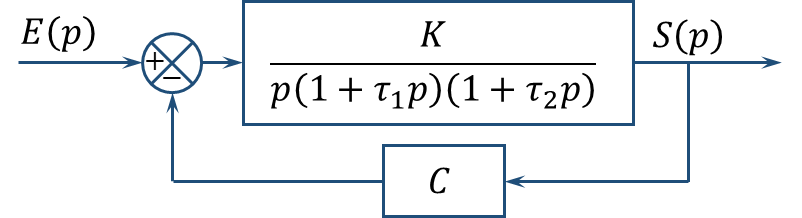
\includegraphics[width=.9\linewidth]{501_01}
\end{center}
 \fi
 
\question{Déterminer la valeur finale de $s(t)$ lorsque l'entrée est un échelon d'amplitude $E_0$.}
\ifprof
\else 
\fi

\question{Déterminer la valeur finale de $s(t)$ lorsque l'entrée est une rampe de pente $k$.}
\ifprof
\else 
\fi


%\question{Réaliser le schéma-blocs.}
%\ifprof
%\begin{figure}[H]
%\centering
%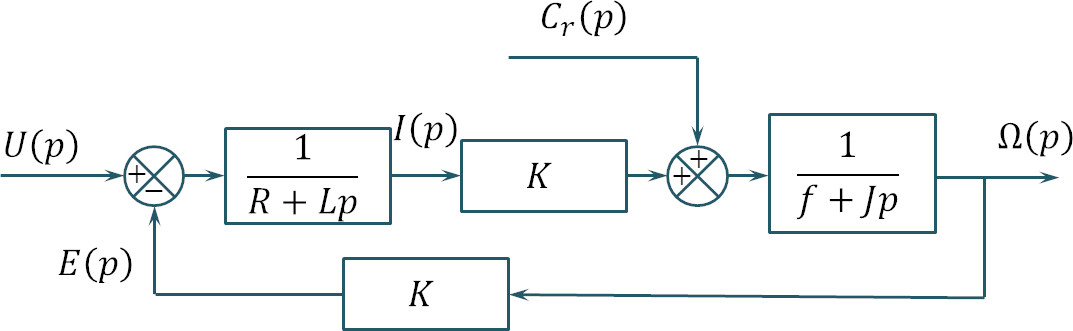
\includegraphics[width=\linewidth]{51_01_c}
%%\caption{Évolution du couple utile en fonction de la vitesse de rotation pour des
%%fréquences de commande de \SI{90}{Hz} à \SI{110}{Hz}. \label{fig_50_04}}
%\end{figure}
%\else
%\fi


 

\ifprof
\else
\begin{flushright}
\footnotesize{Corrigé  voir \ref{C2:03:501}.}
\end{flushright}%
\fi